\documentclass[16pt]{article}
\usepackage{graphicx} 

\graphicspath{{Fig/}{figures/}}

\begin{document}

\centerline{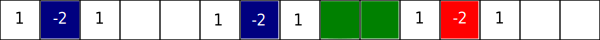
\includegraphics[width=.7\linewidth]{land_sea_decoupling1D}}


\begin{itemize}
\item First 1D, green: land points, everything else: sea point
\item Weights of the discretized Laplacian (in finite difference)
\item Laplacian cannot be computed at the land boundary
\item If 3 consecutive (sea) values are equal $\rightarrow$ Laplacian = 0
\item Laplacian constrain (and the gradient constrain) forces that every values is close to its right and left neighbor
\item This contrain is effecive everywhere except near the boundary
\item The Laplacian couples directly every grid point with its two neighbors,
\item Indirect coupling: two grid points that are separated by some distance as long as they are not separated by land
\item The result is that value of the analysis at the two blue points must be close to each other
\item However, this is not the case of the blue points and the red point
\end{itemize}


\centerline{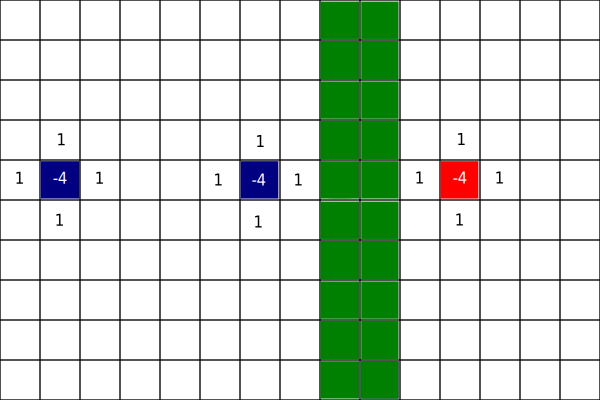
\includegraphics[width=.7\linewidth]{land_sea_decoupling}}

\begin{itemize}
\item In two dimensions, essentially the same procedure.
\item Laplacian couples the field in both spatial directions.
\item DIVA works on a triangular mesh with finite elements, but this basic properties also apply
\end{itemize}

\end{document}
